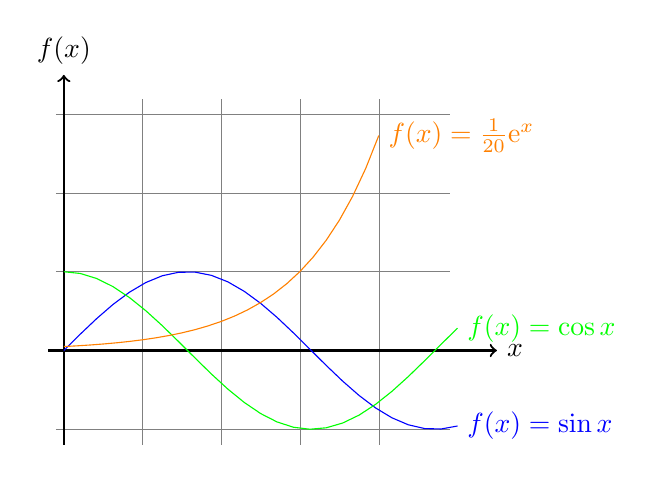
\begin{tikzpicture}[domain=0:5]
  \draw[very thin,color=gray] (-0.1,-1.2) grid (4.9,3.2);
  \draw[->,thick] (-0.2,0) -- (5.5,0) node[right] {$x$};
  \draw[->,thick] (0,-1.2) -- (0,3.5) node[above] {$f(x)$};
  \draw[color=blue] plot (\x,{sin(\x r)}) node[right] {$f(x) = \sin x$};
  \draw[color=green] plot (\x,{cos(\x r)}) node[right] {$f(x) = \cos x$};
  \draw[color=orange,domain=0:4] plot (\x,{0.05*exp(\x)}) node[right] {$f(x) = \frac{1}{20} \mathrm e^x$};
\end{tikzpicture}

